\documentclass[a4paper,10pt]{article}
\usepackage[german]{babel}
\usepackage{ucs}
\usepackage[utf8x]{inputenc}
\usepackage{times}
\usepackage{enumerate}
\usepackage{pstricks}
\usepackage{pst-node}
\usepackage{graphicx}
\usepackage{amsmath}
\usepackage{epsfig}
\usepackage{psfrag}
\usepackage{verbatim}
\usepackage{txfonts}
\usepackage{listings}
\usepackage{hyperref}
\usepackage{svg}
\usepackage{xcolor}
%\usepackage{picins}
\setlength{\textwidth}{160mm}
\setlength{\oddsidemargin}{0mm}
\setlength{\textheight}{280mm}
\setlength{\topmargin}{-20mm}
\pagestyle{empty}
\setlength{\parindent}{0mm}

\usepackage[T1]{fontenc}
\usepackage{listings}
\lstset{
	language=bash,
	basicstyle=\ttfamily,
	showspaces=false,
	basicstyle=\small,
	basewidth = {.44em},
	backgroundcolor=\color{lightgray},
	xleftmargin=.25in,
	xrightmargin=.25in
}
%\textheight 28cm
%\usepackage{latexsym}
%\usepackage{umlaute}


\newcommand{\uebungsnummer}{3}


\begin{document}

\large
%\hfill 
%\begin{figure}[h]
%\scalebox{0.3}{\includegraphics{proaut.eps}}
%\end{figure}

{\textsc Universität Heidelberg}
{\hfill Robotic Games}\\
{\small Lehrstuhl für Automation}
{\hfill \small Wintersemester 2019/2020}%\\
%{\small M.Sc.~Holger~Dieterich}

%\vspace{-8ex}

\begin{center}
{\Large \uebungsnummer. Übung 
\textsc{}}\\
%{\small Ausgabe: 27.~Juni  }
\end{center}

%\smallskip

\begin{center}
\small \it Lernziele: Zugriff Roboter, Fusion
\end{center}

\bigskip
\bigskip

%------------------------------------------------------------------------------

\Large \textbf{1)} Robot \hfill \\ \normalsize



Bisher wurde rein simulativ gearbeitet.
Wir möchten heute den realen Roboter ansteuern.
Um sich mit dem Roboter zu verbinden, müssen wir den richtigen Ros-Master angeben. \\
\textbf{Der ROS-Master-URI muss in jedem neuen Terminal exportiert werden!}
\begin{lstlisting}[language=xml, basicstyle=\small]
export ROS_MASTER_URI=http://192.168.1.199:1234
rostopic list
\end{lstlisting}
Durch \textit{rostopic list} kann geprüft werden ob die Topics des Roboters vorhanden/verbunden sind.

\bigskip
Zusätzlich sollte geprüft werden, dass ROS\_HOSTNAME und ROS\_IP nicht \textit{local} sind.
\begin{lstlisting}[language=xml, basicstyle=\small]
printenv | grep ROS
\end{lstlisting}

\bigskip
Sollten sie lokal sein, bitte die eigene IP verwenden:
\begin{lstlisting}[language=xml, basicstyle=\small]
export ROS_HOSTNAME=192.168.1.XX
export ROS_IP=192.168.1.XX
\end{lstlisting}

\bigskip
Ist alles richtig konfiguriert kann man sich die Messwerte der Ultraschall-Sensoren ansehen.
\begin{lstlisting}[language=xml, basicstyle=\small]
rostopic echo /RosAria/sonar
\end{lstlisting}

\bigskip
Den reale Roboter kann wie in der Simulation mit der Tastatur gesteuert werden.
Die echten Motoren benötigen ledigleich eine zusätzliche Freigabe und der Geschwindigkeitsbefehlt muss zum richtigen Topic publishen. 
\begin{lstlisting}[language=xml, basicstyle=\small]
rosservice call /RosAria/enable_motors
rosrun teleop_twist_keyboard teleop_twist_keyboard.py cmd_vel:=/RosAria/cmd_vel
\end{lstlisting}


\bigskip
Vergleich der Ros-Graphen von Simulation und Experiment:
\begin{lstlisting}[language=xml, basicstyle=\small]
rqt_graph
\end{lstlisting}

Der Graph sollte in etwa so aussehen wie in Abbildung \ref{rosgraph} dargestellt.

\begin{figure}[htbp]
	\centering
	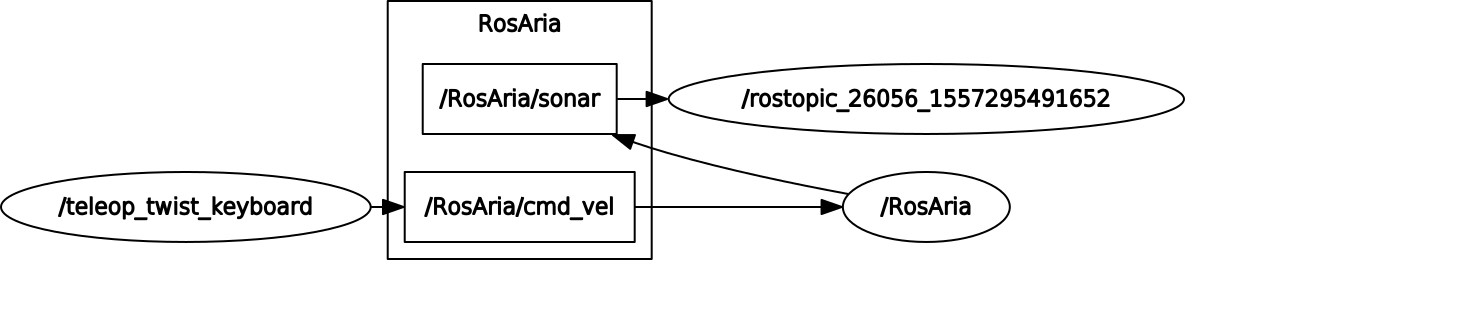
\includegraphics[width=0.8\textwidth]{rosgraph.jpg}
	\caption{ROS Graph}
	\label{rosgraph}
\end{figure}



\newpage

\Large \textbf{2)} Fusion \hfill \\ \normalsize

\end{document}